\documentclass{article}
\usepackage{arxiv}

\usepackage[utf8]{inputenc}
\usepackage[english, russian]{babel}
\usepackage[T1]{fontenc}
\usepackage{url}
\usepackage{booktabs}
\usepackage{amsfonts}
\usepackage{nicefrac}
\usepackage{microtype}
\usepackage{lipsum}
\usepackage{graphicx}
\usepackage{natbib}
\usepackage{doi}
\usepackage{amsmath,amssymb}
\usepackage{hyperref}

\title{Исследование механизмов разрежения нейронных сетей на основе важностей весов}

\author{%
  А.\,В.~Ребриков\thanks{Данная работа выполнена в рамках научно-исследовательской работы (НИР) в Московском физико-техническом институте.}\\
  Физтех-школа прикладной математики и информатики\\
  Московский физико-технический институт (МФТИ)\\
  \texttt{rebryakov.av@phystech.edu} \\
  \And
  А.\,Н.~Безносиков\thanks{Научный руководитель.}\\
  Московский физико-технический институт (МФТИ)\\
  \texttt{beznosikov.an@phystech.edu}
}
\date{}

\renewcommand{\shorttitle}{Разрежение нейронных сетей на основе важностей весов}

\hypersetup{
pdftitle={Исследование механизмов разрежения нейронных сетей на основе важностей весов},
pdfsubject={Разрежение, нейронные сети, DropConnect, важность весов},
pdfauthor={А. В. Ребриков, А. Н. Безносиков},
pdfkeywords={Разрежение, Нейронные сети, DropConnect, Важность весов, Зеркальный спуск, Регуляризация},
}

\begin{document}
\maketitle

\begin{abstract}
В данной работе рассматривается задача регуляризации нейронных сетей путём их разрежения. Традиционные методы, такие как Dropout и DropConnect, «выключают» часть весов случайно, что помогает бороться с переобучением. Мы предлагаем иной подход к определению вероятности выключения весов, основываясь на их \textit{важности} --- оценке вклада конкретных параметров в итоговую функцию ошибки. Эксперименты с ResNet-18 на задаче классификации изображений CIFAR-10 показывают преимущество предлагаемых идей на ранних этапах обучения.
\end{abstract}

\keywords{Разрежение \and Нейронные сети \and DropConnect \and Важность весов \and Регуляризация }

\section{Введение}
В последние годы глубокие нейронные сети достигли значительного прогресса в решении сложных задач компьютерного зрения, обработки естественного языка и многих других областей. Однако большим практическим вызовом остаётся проблема переобучения, а также избыточное количество параметров, которое делает модели ресурсоёмкими и сложными для интерпретации.

Одним из наиболее известных подходов к сдерживанию переобучения является метод \textit{Dropout}~\citep{srivastava2014dropout}, при котором случайным образом «обнуляются» некоторые нейроны на стадии обучения. Аналогичным образом в \textit{DropConnect}~\citep{wan2013regularization} «обнуляются» отдельные веса. Как правило, вероятность зануления задаётся глобально и не учитывает особенности и вклад отдельных весов.

С другой стороны, в последнее время появилось множество работ, исследующих механизмы разрежения нейронных сетей, основанные на важности весов. Например, в работе~\citep{keshari2019guided} предлагается использовать <<силу нейронов>>, т.\,е. оценку их вклада в функцию ошибки, и обучать только наименее сильные.

В данной работе мы предлагаем метод разрежения, использующий \textit{важность} весов, т.\,е. оценку их вклада в функцию ошибки. Для определения важности предлагается зеркальный спуск по соответствующему симплексу для каждого параметра, с дополнительной регуляризацией, препятствующей вырождению в пользу одного веса.

\section{Постановка задачи}
\label{sec:problem}

Рассмотрим задачу обучения нейронной сети на выборке:
\begin{enumerate}
    \item Дано $n$ обучающих примеров $(a_{\text{train}}^i, b_{\text{train}}^i)$, а также $m$ тестовых примеров $(a_{\text{test}}^i, b_{\text{test}}^i)$.
    \item Пусть $x \in X = X_1 \times \dots \times X_L$ --- совокупность весов сети (все слои).
    \item Модель $f(x,a)\colon X \times A \to B$ возвращает результат (например, вектор вероятностей классов).
    \item Функция ошибки $\mathcal{L}(f(x,a^i),b^i)$ суммируется по всем объектам обучающей выборки.
\end{enumerate}

Традиционная постановка задачи обучения нейронной сети:
\begin{equation}
    \frac{1}{n} \sum_{i=1}^{n} \mathcal{L}(f(x, a_{\text{train}}^i), b_{\text{train}}^i) \;\to\; \min_{x \in X}.
\end{equation}

При этом нас дополнительно интересует «обобщающая способность», измеряемая \textit{разностью} качества между тестовой и обучающей выборками (GAP):
\begin{equation}
    \text{GAP} \;=\; \frac{1}{m} \sum_{i=1}^{m} \mathcal{L}\bigl(f(x, a_{\text{test}}^i), b_{\text{test}}^i\bigr)
    \;-\;
    \frac{1}{n} \sum_{i=1}^{n} \mathcal{L}\bigl(f(x, a_{\text{train}}^i), b_{\text{train}}^i\bigr).
\end{equation}

Целью регуляризации служит снижение риска переобучения, то есть уменьшение величины GAP.

\section{Определение важности весов и разрежение}
\label{sec:importance}

Для построения механизма разрежения на основе \textit{важности} весов необходимо:
\begin{enumerate}
    \item Определить меру важности для каждого веса $x_i$.
    \item На основе этой меры задавать вероятности «включения» (или «выключения») весов при DropConnect.
    \item В случае необходимости сочетать полученную схему с классическим \textit{DropConnect} или другими известными техниками.
\end{enumerate}

\subsection{Зеркальный спуск на симплексе}
В работе предлагается найти распределение важности $w$ размерности, совпадающей с количеством весов. Для этого решается задача:
\begin{equation}
    \mathcal{L}\bigl(f(x - w \odot (\gamma \nabla f(x)), a_{\text{train}}), b_{\text{train}}\bigr)
    \;\to\; \min_{w}, 
\end{equation}
где $w$ лежит на соответствующем симплексе, умноженном на количество весов, $\gamma$ --- параметр «шага». Решение реализуется методом зеркального спуска с регуляризацией в виде KL-дивергенции:
\begin{equation}
    R(w) \;=\; \mathrm{KL}(w \,\|\, \boldsymbol{u}),
\end{equation}
где $\boldsymbol{u}$ --- равномерное распределение (в данном случае, все компоненты равны $1$). Это препятствует «вырождению» в пользу одного веса, одновременно позволяя различать важные и менее важные веса.

\section{Применение DropConnect на основе важности}
\label{sec:dropconnect}

\textit{DropConnect}~\citep{wan2013regularization} предполагает, что в процессе обучения каждая компонента $x_i$ (вес сети) «выключается» с некоторой вероятностью $p$. Мы же можем задать это $p$ как функцию от найденной важности $w_i$. Например,
\[
    p_i = 1 - \alpha \, w_i \quad \text{(или наоборот } p_i = \alpha \, w_i \text{)}, 
\]
где $\alpha$ --- параметр, задающий уровень разрежения.

Далее обучения сети проходит с учётом того, что веса выбираются случайно в соответствии с вероятностями $p_i$.

\section{Эксперименты}
\label{sec:experiments}

\subsection{Настройка экспериментов}
Эксперименты проводились на датасете CIFAR-10 с помощью архитектуры ResNet-18. Рассматривались следующие методы:
\begin{itemize}
    \item \textbf{baseline:} обучение без разрежения;
    \item \textbf{impacts:} обучение с DropConnect, где вероятность задаётся на основе важностей весов;
    \item \textbf{impacts+regularization:} то же, что impacts, но с дополнительной регуляризацией KL-дивергенции, препятствующей вырождению распределения важности;
    \item \textbf{dropconnect:} классический DropConnect с фиксированной вероятностью выключения.
\end{itemize}

Во всех трёх вариантах с разрежением старались «выключать» одинаковое количество весов, чтобы иметь сопоставимые условия.

\subsection{Результаты}
На Рисунке~\ref{fig:hist} показаны гистограммы важных весов с регуляризацией. При отсутствии регуляризации наблюдалось «выделение» единственного веса с максимальной важностью, что приводило к вырожденной ситуации. С KL-регуляризацией распределение более плавное, сохраняя «группу» наиболее важных весов.

\begin{figure}[h]
    \centering
    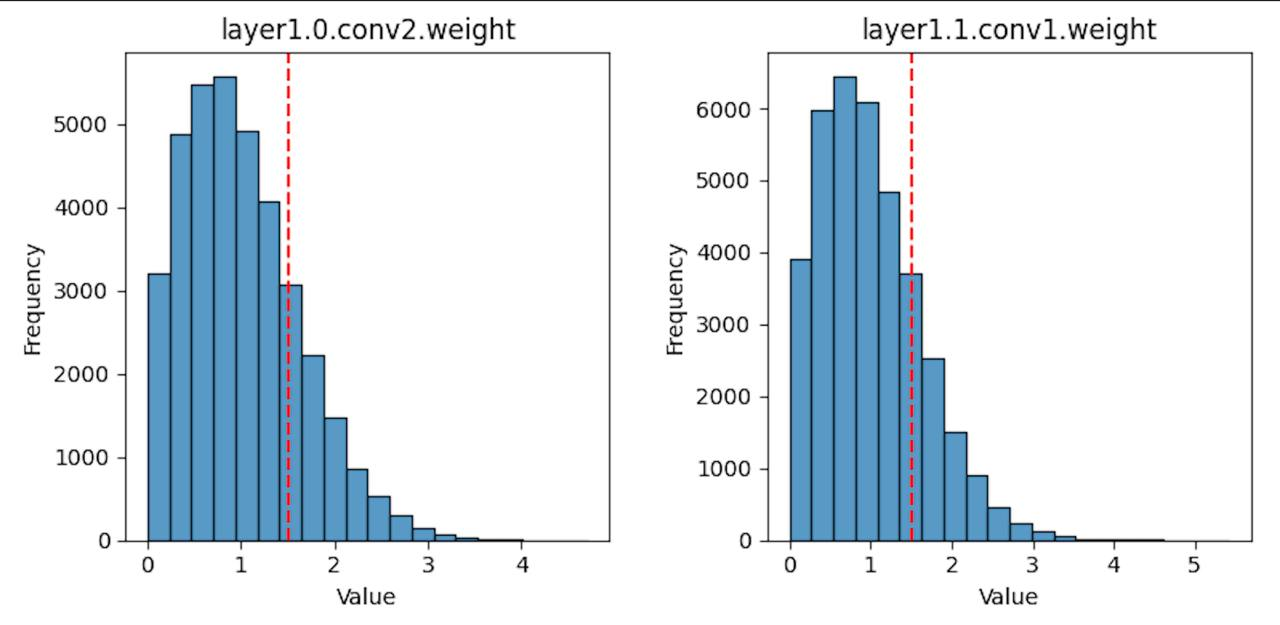
\includegraphics[width=0.6\textwidth]{../figures/impacts.jpeg}
    \caption{Гистограммы важностей весов с регуляризацией.}
    \label{fig:hist}
\end{figure}

На Рисунке~\ref{fig:exp} представлены графики обучения (точность на валидации и ошибка), показывающие, что на ранних этапах метод impacts+regularization даёт лучший результат по сравнению с классическим DropConnect.

\begin{figure}[h]
    \centering
    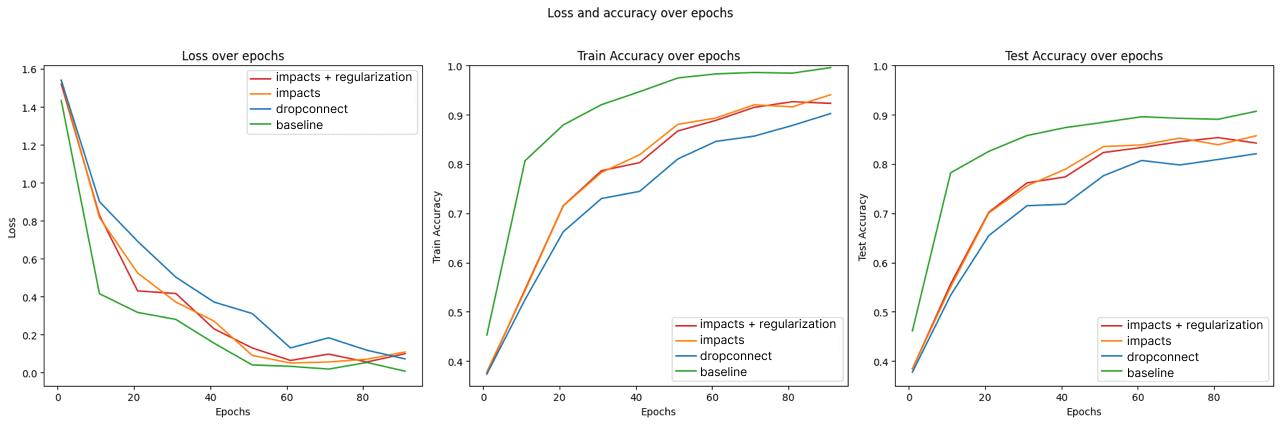
\includegraphics[width=0.9\textwidth]{../figures/exp.png}
    \caption{Сходимость на ранних эпохах обучения ResNet-18 с разрежением в вариантах baseline, dropconnect, impacts и impacts+regularization.}
    \label{fig:exp}
\end{figure}

\section{Выводы и дальнейшие исследования}
\label{sec:conclusion}

В работе представлен новый подход к регуляризации нейронных сетей, основанный на вычислении важности весов и применении DropConnect с вероятностями, зависящими от важности. Эксперименты показали преимущество такого подхода на ранних этапах обучения по сравнению с классическими методами.

\textbf{Основные результаты:}
\begin{enumerate}
    \item Предложен метод определения важности весов с помощью зеркального спуска на симплексе и KL-регуляризации.
    \item Показано, что основанный на важностях метод DropConnect даёт более высокое качество в начальной фазе обучения.
    \item Сохранение «небольшой группы важных весов» выглядит более разумным, чем равномерное вероятностное выключение всех весов.
\end{enumerate}

\textbf{Перспективы:}
\begin{itemize}
    \item Исследовать устойчивость и поведение предлагаемого подхода на поздних этапах обучения.
    \item Рассмотреть комбинирование с другими методами разрежения, включая различные эвристики пороговых значений весов, L1-регуляризацию и т.\,д.
    \item Применение на более сложных архитектурах и задачах .
\end{itemize}

\section*{Благодарности}
Авторы благодарят МФТИ за предоставленную вычислительную инфраструктуру и поддержку исследований.

\bibliographystyle{unsrtnat}
\bibliography{references}
\nocite{*}

\end{document}
